\documentclass[11pt]{article}

\usepackage[utf8]{inputenc}
\usepackage[T1]{fontenc}
\usepackage{lmodern}
\usepackage[margin=0.9in]{geometry}
\usepackage{amsmath,amssymb,mathtools,bm}
\usepackage{booktabs,tabularx,array,multirow}
\usepackage{graphicx}
\usepackage{microtype}
\usepackage{xcolor}
\usepackage{enumitem}
\usepackage{hyperref}
\usepackage{cleveref}
\usepackage{tikz}
\usepackage{float}
\usepackage{placeins}
\usetikzlibrary{arrows.meta,positioning,calc,fit,shapes.geometric,decorations.pathreplacing}

\hypersetup{
  colorlinks=true,
  linkcolor=blue!45!black,
  citecolor=blue!45!black,
  urlcolor=blue!45!black
}

\newcommand{\E}{\mathbb{E}}
\newcommand{\Var}{\operatorname{Var}}
\newcommand{\Cov}{\operatorname{Cov}}
\newcommand{\diag}{\operatorname{diag}}
\newcommand{\R}{\mathbb{R}}
\newcommand{\pos}[1]{\left[#1\right]_+}
\newcommand{\given}{\,\middle|\,}
\newcommand{\norm}[1]{\left\lVert#1\right\rVert}
\newcommand{\trans}{\mathsf T}

\title{\textbf{Hierarchical Parzen ICA for Neural Imaging}\\
Background Reconstruction, Noisy Source Separation, and Stable Real-Time Inference}
\author{
Raul Valle \and Jos\'e C. Principe\\
Department of Electrical and Computer Engineering\\
University of Florida
}
\date{Working methods manuscript --- July 29, 2026}

\begin{document}
\maketitle

\begin{abstract}
NeuRev experiments have established two complementary facts. First, adjacent-frame
InfoMax and Cauchy--Schwarz Parzen separation recover a direction nearly identical
to temporal subtraction, showing that pairwise ICA naturally separates a
persistent common mode from change. Second, amplitude-preserving representations
are currently more useful than derivative-only features: an offline stable
AR(1) smoother and low-rank amplitude PCA improve known-label recovery, whereas
raw and latent differences, model-aware dynamic drive, and filter innovation
underperform. These results motivate a hierarchical rather than monolithic source
model. Stage~1 uses batch or stochastic Parzen ICA on aligned frame pairs to
identify and reconstruct a background-like common component while preserving an
amplitude residual. Stage~2 treats overlapping residual patches as noisy linear
mixtures, estimates observation-noise covariance from quiet residuals, performs
noise-corrected subspace selection, and fits a local noisy Parzen ICA model. The
source density is represented by a Gaussian Parzen dictionary convolved with the
projected additive-noise distribution; this yields both a noise-aware score
function for stochastic demixing updates and an analytic posterior mean for
clean-source estimation. Structured components are subsequently classified as
neural signal, artifact, or unresolved using spatial localization, annularity,
temporal coherence, recurrence, motion correlation, and stability. We specify
identifiability limitations, numerical and scientific stability requirements, a
real-time two-timescale architecture, a falsification-oriented synthetic and
semi-synthetic program, and mandatory visual and quantitative outputs centered
on decomposition closure, background--signal--artifact--noise leakage, event
preservation, residual validity, downstream detection, and latency.
\end{abstract}

\section{Canonical problem statement}

The desired scientific result is not simply a smooth movie. It is a decomposition
whose channels have distinct meanings:
\begin{equation}
Y_t(p)
=
B_t(p)+S_t(p)+A_t(p)+N_t(p),
\label{eq:fourway}
\end{equation}
where $B$ is background-like structure, $S$ is accepted neural dynamics, $A$ is
structured artifact, and $N$ is stochastic measurement noise. A user-facing
three-way view may combine $A+N$ as residual uncertainty, but the internal
four-way representation is necessary: motion edges, saturation, and coherent
acquisition errors are not ordinary noise and should not be promoted to neural
signal.

The hierarchy proposed here is
\begin{equation}
Y
\xrightarrow{\text{Stage 1}}
\widehat B+R,
\qquad
R
\xrightarrow{\text{Stage 2}}
\widehat S+\widehat A+\widehat N.
\end{equation}
The end-to-end closure is
\begin{equation}
E_{\mathrm{closure}}
=
Y-\widehat B-\widehat S-\widehat A-\widehat N.
\end{equation}
A decomposition is not credible unless $E_{\mathrm{closure}}$ is small and the
energy assigned to each channel is scientifically appropriate.

\begin{figure}[H]
\centering
\resizebox{\textwidth}{!}{%
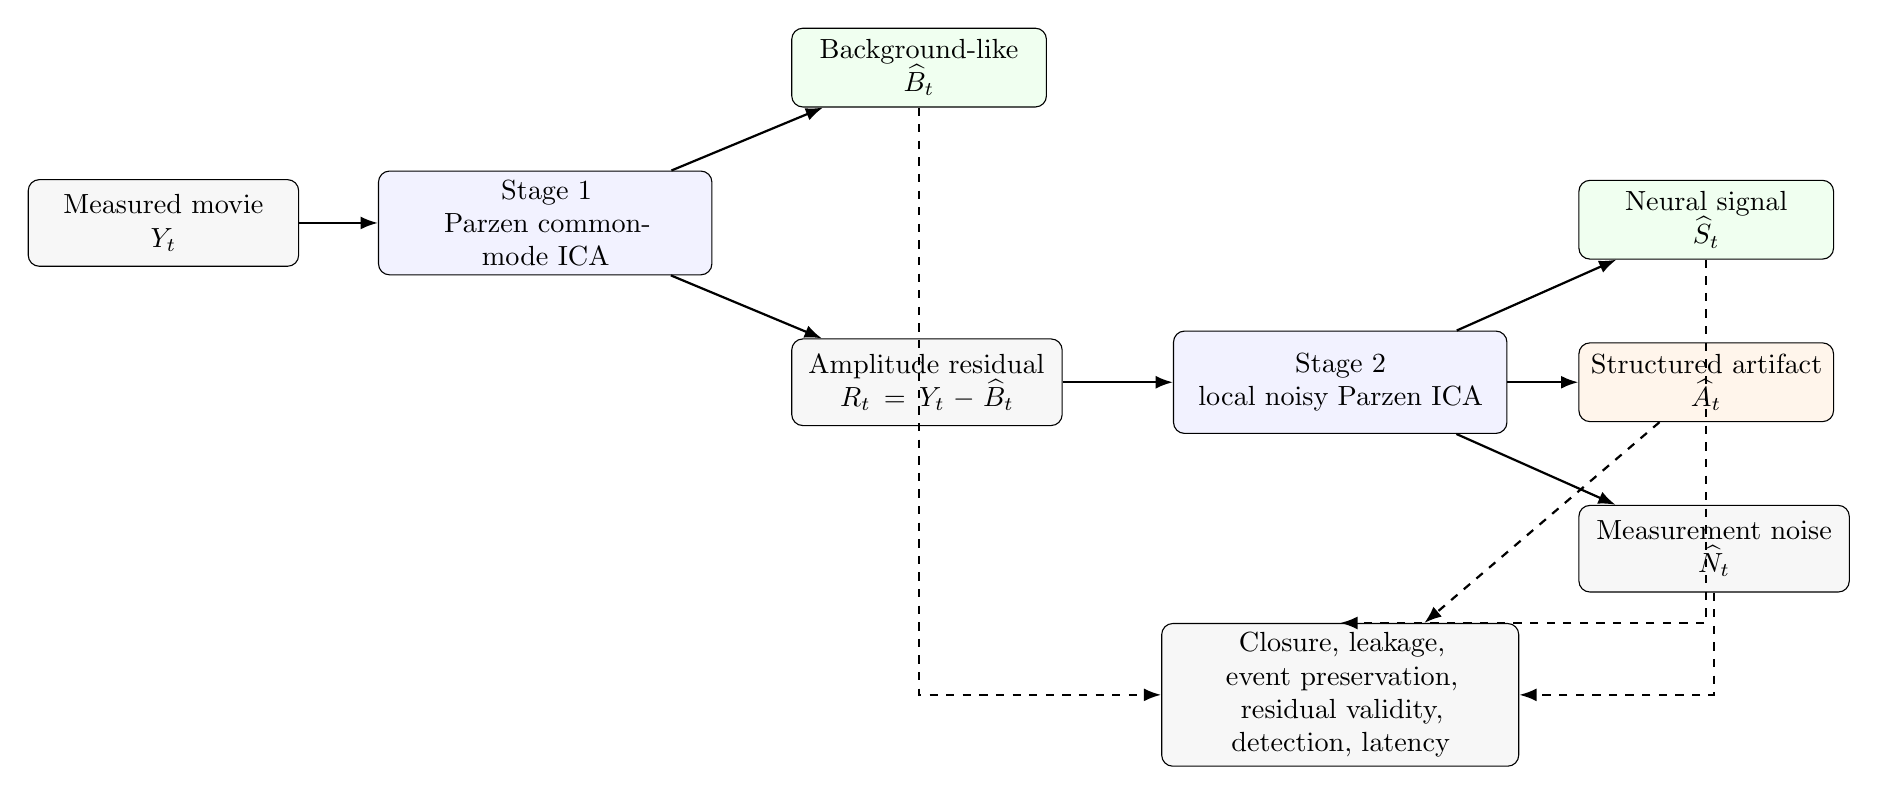
\begin{tikzpicture}[
  node distance=8mm and 10mm,
  box/.style={draw, rounded corners, align=center, minimum height=11mm,
              text width=32mm, fill=black!3},
  stage/.style={draw, rounded corners, align=center, minimum height=13mm,
                text width=40mm, fill=blue!5},
  output/.style={draw, rounded corners, align=center, minimum height=10mm,
              text width=30mm, fill=green!6},
  artifact/.style={draw, rounded corners, align=center, minimum height=10mm,
              text width=30mm, fill=orange!8},
  arrow/.style={-{Latex[length=2.2mm]}, thick}
]
\node[box] (raw) {Measured movie\\$Y_t$};
\node[stage, right=of raw] (s1) {Stage 1\\Parzen common-mode ICA};
\node[output, above right=8mm and 10mm of s1] (bg) {Background-like\\$\widehat B_t$};
\node[box, below right=8mm and 10mm of s1] (res) {Amplitude residual\\$R_t=Y_t-\widehat B_t$};
\node[stage, right=14mm of res] (s2) {Stage 2\\local noisy Parzen ICA};
\node[output, above right=9mm and 9mm of s2] (sig) {Neural signal\\$\widehat S_t$};
\node[artifact, right=9mm of s2] (art) {Structured artifact\\$\widehat A_t$};
\node[box, below right=9mm and 9mm of s2] (noise) {Measurement noise\\$\widehat N_t$};
\node[box, text width=43mm, below=24mm of s2] (metrics) {Closure, leakage, event preservation,\\residual validity, detection, latency};

\draw[arrow] (raw) -- (s1);
\draw[arrow] (s1) -- (bg);
\draw[arrow] (s1) -- (res);
\draw[arrow] (res) -- (s2);
\draw[arrow] (s2) -- (sig);
\draw[arrow] (s2) -- (art);
\draw[arrow] (s2) -- (noise);
\draw[arrow, dashed] (bg) |- (metrics.west);
\draw[arrow, dashed] (sig) |- (metrics.north);
\draw[arrow, dashed] (art) -- (metrics);
\draw[arrow, dashed] (noise) |- (metrics.east);
\end{tikzpicture}%
}
\caption{The proposed scientific order. Stage~1 reconstructs rather than merely
forwards a derivative component. Stage~2 explicitly models additive noise and
retains coherent non-neural residuals as artifacts.}
\label{fig:pipeline}
\end{figure}

\section{What the present NeuRev evidence implies}

The current repository provides four motivating observations.

\paragraph{Pairwise ICA became a derivative.}
For adjacent samples
\begin{equation}
\bm x_t(p)=
\begin{bmatrix}I_{t-1}(p)&I_t(p)\end{bmatrix}^{\trans},
\end{equation}
persistent structure lies near $[1,1]^{\trans}$ and its orthogonal change
direction is $[-1,1]$. Existing InfoMax and CS-Parzen fits recovered effective
directions almost collinear with subtraction. This is useful evidence that the
pair contains a common/background-like mode, but it does not identify every
physical source.

\paragraph{Change alone did not replace amplitude.}
Fixed/adaptive differences and pairwise ICA were useful as onset or change
evidence but did not improve the frozen Raw Direct detector under the tested
additive and gating rules. Strong gates removed slowly evolving calcium
activity.

\paragraph{Denoised amplitude helped.}
A stable shared AR(1) offline smoother improved known-label recovery over Raw
Direct, while raw and latent differences, positive dynamic drive, and
standardized filter innovation underperformed. The useful representation was
latent amplitude, not post-denoising differencing.

\paragraph{Low rank helped only modestly and high-rank ICA destabilized.}
Amplitude PCA at rank eight produced a small provisional fixed-budget gain.
Rank-16 spatial ICA was stable but did not win at fixed budget; rank-64 ICA hit
the iteration cap and showed poor seed stability. This argues for bounded local
rank and explicit stability gates.

The new hierarchy therefore preserves the common-versus-change idea, but the
Stage~1 output is an amplitude residual, and the Stage~2 model is local,
noise-aware, and rank constrained.

\section{Identifiability boundary}

The decomposition in \cref{eq:fourway} is not uniquely identifiable without
structural assumptions. Two limitations matter immediately.

\subsection{Two observations identify at most two aggregate directions}

For one pixel and two adjacent frames, the data contain background, previous and
current neural state, previous and current noise, and possible motion. A
$2\times2$ ICA can recover at most two aggregate components. Stage~1 should
therefore be interpreted as
\begin{equation}
\text{common/background-like mode}
\quad\big|\quad
\text{dynamic residual mode},
\end{equation}
not as a complete physical decomposition.

\subsection{Noise is not an ordinary ICA source}

For a noisy mixture
\begin{equation}
\bm r_t=A\bm s_t+\bm n_t,
\end{equation}
Gaussian noise does not generally define a unique ICA direction. After
whitening, isotropic Gaussian noise is rotation invariant. The correct Stage~2
task is to identify reproducible structured sources under an additive-noise
model and leave the remaining unexplained variation as residual uncertainty.
Noisy-ICA theory also distinguishes estimation of the mixing matrix from
minimum-noise source recovery; naive inversion is not automatically optimal
\cite{voss2015pegi}.

\section{Stage 1: Parzen common-mode separation}

\subsection{Pair construction and gain correction}

For lag $k$, define
\begin{equation}
\bm x_t(p)=
\begin{bmatrix}
I_{t-k}(p)\\
I_t(p)
\end{bmatrix}.
\label{eq:pair}
\end{equation}
The initial reference uses $k=1$. A robust gain model may estimate
\begin{equation}
I_t(p)\approx \alpha_t I_{t-k}(p)+d_t(p),
\end{equation}
so that the gain-adjusted common and differential directions are approximately
\begin{equation}
\bm c_t=
\begin{bmatrix}1\\ \alpha_t\end{bmatrix},
\qquad
\bm d_t=
\begin{bmatrix}-\alpha_t\\1\end{bmatrix}.
\end{equation}
The gain coefficient $\alpha_t$ is an observation parameter and must not be
confused with a calcium decay coefficient.

\subsection{Stable whitening}

Center and whiten bounded spatial samples:
\begin{equation}
\bm z_t(p)=Q_t[\bm x_t(p)-\bm\mu_t].
\end{equation}
The covariance eigendecomposition must use a floor and report its condition
number. If the second eigenvalue is below the declared floor, the pair is
unidentifiable and no arbitrary ICA component should be emitted.

\subsection{Batch CS-Parzen reference}

The existing NeuRev reference estimates independence with a Gaussian-Parzen
Cauchy--Schwarz divergence. For densities $p$ and $q$,
\begin{equation}
D_{\mathrm{CS}}(p,q)
=-\log
\frac{\left(\int p(u)q(u)\,du\right)^2}
{\int p(u)^2\,du\int q(u)^2\,du}.
\end{equation}
For two whitened outputs, the demixer is an orthogonal rotation, so a bounded
angle search supplies an auditable reference. Kernel work must use deterministic
subsamples and blockwise evaluation.

\subsection{Stochastic Parzen score-function ICA}

Stochastic information-gradient methods were introduced to reduce the cost of
online entropy manipulation from all-pairs estimation toward bounded stochastic
updates \cite{erdogmus2003sig}. For component $j$, maintain a dictionary
$\{c_{jm}\}_{m=1}^{M}$ and Gaussian bandwidth $h_j$:
\begin{equation}
\widehat p_j(y)
=
\frac1M\sum_{m=1}^{M}
\mathcal N(y;c_{jm},h_j^2).
\end{equation}
The posterior responsibility of center $m$ is
\begin{equation}
\alpha_{jm}(y)
=
\frac{\mathcal N(y;c_{jm},h_j^2)}
{\sum_{\ell}\mathcal N(y;c_{j\ell},h_j^2)},
\end{equation}
and the negative score is
\begin{equation}
\psi_j(y)
=
-\frac{\partial}{\partial y}\log\widehat p_j(y)
=
\frac{y-\sum_m\alpha_{jm}(y)c_{jm}}{h_j^2}.
\label{eq:clean-score}
\end{equation}
A natural-gradient-style update is
\begin{equation}
W^{+}
=
\operatorname{decorrelate}
\left(
W+\eta
[I-\bm\psi(\bm y)\bm y^{\trans}]W
\right),
\label{eq:natural-update}
\end{equation}
where the implementation must freeze a sign convention and verify the update
against finite differences and the batch objective on small fixtures. Hild,
Erdogmus, and Principe analyzed modified stochastic estimators that accommodate
both super- and sub-Gaussian sources and exploit temporal diversity
\cite{hild2006entropy}.

The dictionary is bounded. New centers should be posterior or filtered source
samples, not an unbounded history of every observation. Minimum separation,
replacement policy, age, usage, and bandwidth bounds must be recorded.

\subsection{Identifying the background-like component}

A near-zero \emph{mean} derivative is insufficient because zero-mean noise also
has that property. Use normalized derivative energies:
\begin{align}
E_1(j)
&=
\frac{\operatorname{median}_{t,p}
[(y_{j,t}(p)-y_{j,t-1}(p))^2]}
{\Var_{t,p}(y_{j,t}(p))+\epsilon},\\
E_2(j)
&=
\frac{\operatorname{median}_{t,p}
[(y_{j,t}(p)-2y_{j,t-1}(p)+y_{j,t-2}(p))^2]}
{\Var_{t,p}(y_{j,t}(p))+\epsilon}.
\end{align}
For independent white noise with variance $\sigma^2$,
\begin{equation}
\Var(\Delta n_t)=2\sigma^2,
\qquad
\Var(\Delta^2n_t)=6\sigma^2,
\end{equation}
so derivative energy separates static structure from noise more effectively than
mean derivative.

The component score should also use:
\begin{itemize}[leftmargin=*]
\item cosine similarity to the common and differential directions;
\item spatial total variation or high-frequency mass;
\item spatial support/broadness;
\item correlation with global frame intensity;
\item continuity across updates;
\item event-versus-quiet modulation for reporting, not held-out selection.
\end{itemize}
A small score margin must return \texttt{unresolved}. This protects slow calcium
activity, which may have low derivative energy over adjacent frames.

\begin{figure}[H]
\centering
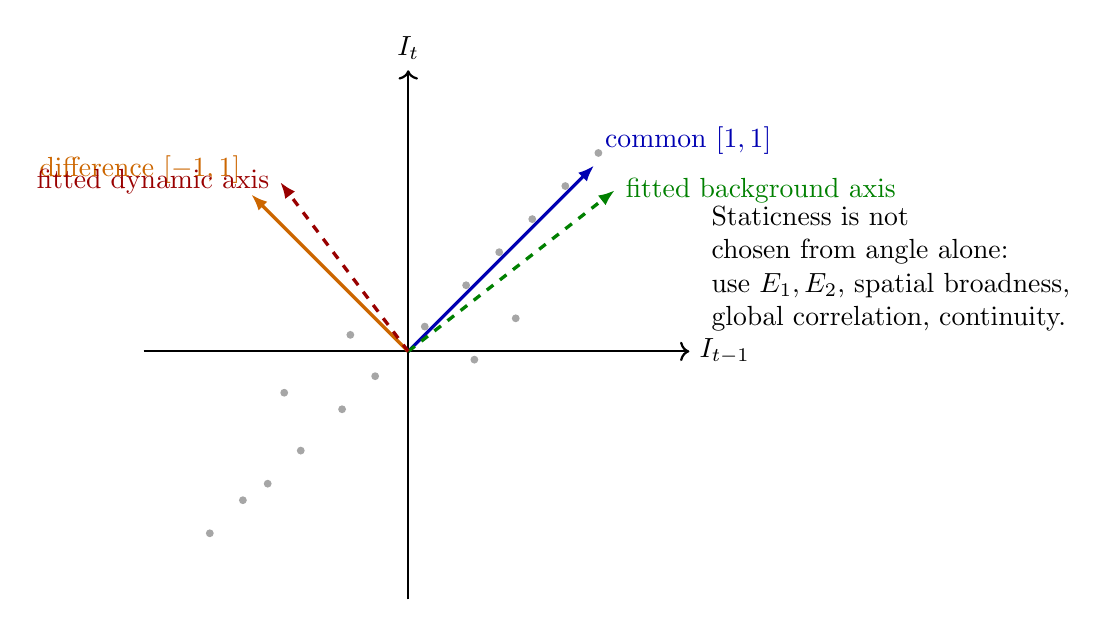
\begin{tikzpicture}[scale=1.05,
  axis/.style={->,thick},
  vec/.style={-{Latex[length=2.1mm]},very thick},
  point/.style={circle,fill=black!35,inner sep=1pt}]
\draw[axis] (-3.2,0)--(3.4,0) node[right] {$I_{t-1}$};
\draw[axis] (0,-3.0)--(0,3.4) node[above] {$I_t$};
\foreach \x/\y in {-2.4/-2.2,-2.0/-1.8,-1.7/-1.6,-1.3/-1.2,-0.8/-0.7,-0.4/-0.3,0.2/0.3,0.7/0.8,1.1/1.2,1.5/1.6,1.9/2.0,2.3/2.4,1.3/0.4,0.8/-0.1,-0.7/0.2,-1.5/-0.5}
  \node[point] at (\x,\y) {};
\draw[vec,blue!70!black] (0,0)--(2.25,2.25) node[above right] {common $[1,1]$};
\draw[vec,orange!80!black] (0,0)--(-1.9,1.9) node[above left] {difference $[-1,1]$};
\draw[vec,green!50!black,dashed] (0,0)--(2.5,1.95) node[right] {fitted background axis};
\draw[vec,red!60!black,dashed] (0,0)--(-1.55,2.05) node[left] {fitted dynamic axis};
\node[align=left,anchor=west] at (3.55,1.0) {Staticness is not\\chosen from angle alone:\\use $E_1,E_2$, spatial broadness,\\global correlation, continuity.};
\end{tikzpicture}
\caption{Stage~1 geometry. Persistent anatomy produces an elongated common mode;
change and noise occupy the orthogonal direction. The actual component label must
combine geometry with temporal and spatial diagnostics.}
\label{fig:stage1-geometry}
\end{figure}

\subsection{Background reconstruction and amplitude residual}

Let
\begin{equation}
\bm y=WQ(\bm x-\bm\mu).
\end{equation}
If $W$ is orthogonal after whitening,
\begin{equation}
\bm x
=
\bm\mu+Q^{\dagger}W^{\trans}\bm y.
\end{equation}
Set the dynamic component to zero to form
$\widehat{\bm x}^{(B)}$. The current-frame background is
\begin{equation}
\widehat B_t(p)=
[\widehat{\bm x}^{(B)}_t(p)]_2,
\end{equation}
and the Stage~1 residual is
\begin{equation}
R_t(p)=I_t(p)-\widehat B_t(p).
\label{eq:stage1-residual}
\end{equation}
Equation~\eqref{eq:stage1-residual} is central: Stage~2 receives an
amplitude-preserving residual, not only the derivative-like ICA output.

\section{Stage 2: local noisy Parzen ICA}

\subsection{Patchwise noisy mixture}

For overlapping patch $k$ with $P$ pixels,
\begin{equation}
\bm r_t^{(k)}
=A_k\bm s_t^{(k)}+\bm a_t^{(k)}+\bm n_t^{(k)}.
\label{eq:noisy-patch}
\end{equation}
The patch provides multiple sensors; this is necessary because one scalar pixel
trace cannot identify multiple latent sources and noise. Local patches also
exploit neighboring-pixel coherence and bound the component rank.

\subsection{Noise estimation and signal-subspace selection}

Estimate quiet residual covariance $\widehat\Sigma_n$ using a diagonal,
shrinkage, or gated low-rank-plus-diagonal model. The structured covariance is
\begin{equation}
\widehat\Sigma_s
=
\Pi_{\succeq0}
(\widehat\Sigma_r-\widehat\Sigma_n),
\label{eq:noise-corrected-cov}
\end{equation}
where negative eigenvalues are clipped. Select only positive modes that exceed
noise-floor and temporal-block stability thresholds. This is a required control:
ordinary PCA whitening and noise-corrected whitening must be compared.

Let $Q$ project and whiten the retained subspace:
\begin{equation}
\widetilde{\bm r}_t=Q\bm r_t,
\qquad
\bm y_t=W\widetilde{\bm r}_t.
\end{equation}
The projected noise covariance is
\begin{equation}
\Sigma_{\widetilde n}=Q\widehat\Sigma_nQ^{\trans}.
\end{equation}
For output row $\bm w_j^{\trans}$,
\begin{equation}
\nu_j^2=\bm w_j^{\trans}
\Sigma_{\widetilde n}\bm w_j.
\label{eq:projected-noise}
\end{equation}

\subsection{Noise-convolved Parzen density}

Assume
\begin{equation}
y_j=s_j+\eta_j,
\qquad
\eta_j\sim\mathcal N(0,\nu_j^2).
\end{equation}
Represent the latent source density by
\begin{equation}
\widehat p_{s_j}(s)
=
\frac1M\sum_{m=1}^{M}
\mathcal N(s;c_{jm},h_j^2).
\label{eq:source-parzen}
\end{equation}
Gaussian convolution gives the observed noisy density
\begin{equation}
\widehat p_{y_j}(y)
=
\frac1M\sum_{m=1}^{M}
\mathcal N(y;c_{jm},h_j^2+\nu_j^2).
\label{eq:noisy-parzen}
\end{equation}
The source bandwidth $h_j$ and observation-noise variance $\nu_j^2$ have
different meanings and must not be collapsed into one unconstrained kernel
parameter.

Define
\begin{equation}
\alpha_{jm}(y)
=
\frac{\mathcal N(y;c_{jm},h_j^2+\nu_j^2)}
{\sum_{\ell}\mathcal N(y;c_{j\ell},h_j^2+\nu_j^2)},
\end{equation}
then
\begin{equation}
\psi_j(y)
=
-\frac{\partial}{\partial y}\log\widehat p_{y_j}(y)
=
\frac{y-\sum_m\alpha_{jm}(y)c_{jm}}
{h_j^2+\nu_j^2}.
\label{eq:noisy-score}
\end{equation}
Substituting \cref{eq:noisy-score} into the bounded natural update
\cref{eq:natural-update} yields the proposed stochastic noisy Parzen ICA lane.
An earlier adaptive-filter study used an augmented ICA model, Parzen density
estimation, and stochastic information gradient to separate a signal from noisy
observations by maximizing independence rather than minimizing mean-square error
\cite{yang2007adaptive}. The present proposal differs in its spatial patch model,
explicit noise-convolved source density, posterior source reconstruction, and
four-way residual qualification.

\subsection{Posterior clean-source estimate}

For prior component $m$,
\begin{equation}
s_j\sim\mathcal N(c_{jm},h_j^2),
\qquad
y_j=s_j+\eta_j.
\end{equation}
Gaussian conditioning gives
\begin{equation}
\mu_{jm}(y)
=
\E[s_j\mid y_j=y,m]
=
\frac{\nu_j^2c_{jm}+h_j^2y}
{h_j^2+\nu_j^2}.
\end{equation}
The mixture posterior mean is
\begin{equation}
\widehat s_j(y)
=
\sum_m\alpha_{jm}(y)\mu_{jm}(y).
\label{eq:posterior-mean}
\end{equation}
This is a principled denoised source amplitude. The Parzen dictionary should be
updated with posterior source estimates, not raw noisy outputs, to avoid simply
learning the noise-broadened distribution.

\begin{figure}[H]
\centering
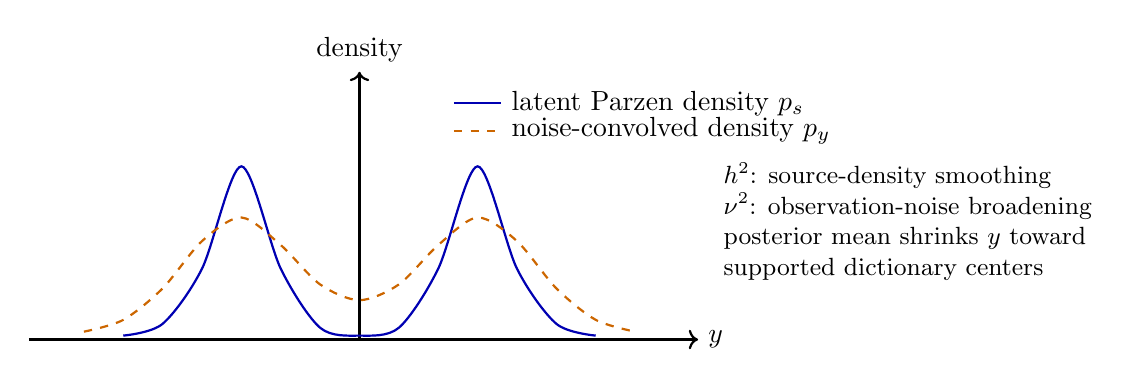
\begin{tikzpicture}[
  x=1.0cm,y=1.0cm,
  axis/.style={->,thick},
  curve/.style={thick},
  note/.style={align=left,font=\small}]
\draw[axis] (-4.2,0)--(4.3,0) node[right] {$y$};
\draw[axis] (0,0)--(0,3.4) node[above] {density};
\draw[curve,blue!70!black]
  plot[smooth] coordinates {(-3,0.05)(-2.5,0.2)(-2,0.9)(-1.5,2.2)(-1,0.9)(-0.5,0.15)(0,0.05)(0.5,0.15)(1,0.9)(1.5,2.2)(2,0.9)(2.5,0.2)(3,0.05)};
\draw[curve,orange!80!black,dashed]
  plot[smooth] coordinates {(-3.5,0.1)(-3,0.25)(-2.5,0.65)(-2,1.25)(-1.5,1.55)(-1,1.2)(-0.5,0.7)(0,0.5)(0.5,0.7)(1,1.2)(1.5,1.55)(2,1.25)(2.5,0.65)(3,0.25)(3.5,0.1)};
\draw[blue!70!black,thick] (1.2,3.0)--(1.8,3.0) node[right,black] {latent Parzen density $p_s$};
\draw[orange!80!black,thick,dashed] (1.2,2.65)--(1.8,2.65) node[right,black] {noise-convolved density $p_y$};
\node[note,anchor=west] at (4.5,1.5) {$h^2$: source-density smoothing\\$\nu^2$: observation-noise broadening\\posterior mean shrinks $y$ toward\\supported dictionary centers};
\end{tikzpicture}
\caption{Schematic, not experimental data. Gaussian noise broadens the observed
Parzen density analytically. The same model supplies the score function used for
demixing and the posterior mean used for source denoising.}
\label{fig:noisy-density}
\end{figure}

\subsection{Patch reconstruction}

Map the posterior sources back to patch coordinates:
\begin{equation}
\widehat{\bm r}^{(S)}_t
=Q^{\dagger}W^{-1}\widehat{\bm s}_t.
\end{equation}
For an orthogonal $W$, $W^{-1}=W^{\trans}$; otherwise use a checked
pseudoinverse and report its condition number. Overlapping patches are combined
with a declared Hann or Tukey window and normalization.

The preliminary residual is
\begin{equation}
\bm e_t=\bm r_t-\widehat{\bm r}^{(S)}_t.
\end{equation}
It is not yet measurement noise.

\section{Neural signal, artifact, and noise qualification}

Noisy ICA identifies structured components but does not know which components
are neurons. Qualify each component using:
\begin{itemize}[leftmargin=*]
\item spatial localization, compactness, and connectedness;
\item annular or membrane-like morphology;
\item local temporal coherence;
\item event-versus-quiet robust modulation;
\item recurrence across windows;
\item alignment and stability across seeds and patch offsets;
\item correlation with spatial gradients or motion fields;
\item saturation/bright-artifact overlap;
\item posterior denoising gain and residual reduction.
\end{itemize}
The output class is one of
\begin{equation}
\{\texttt{accepted\_neural},
\texttt{structured\_artifact},
\texttt{unresolved}\}.
\end{equation}
Only accepted components form $\widehat S$. Coherent rejected components form
$\widehat A$.

The remaining residual may be called $\widehat N$ only if it exhibits:
\begin{itemize}[leftmargin=*]
\item low nonzero-lag temporal autocorrelation;
\item low spatial correlation beyond the optical scale;
\item little event-triggered energy at known neurons;
\item low correlation with motion/edge maps;
\item stable quiet statistics;
\item variance consistent with intensity.
\end{itemize}
Fluorescence measurements often contain signal-dependent shot noise plus
approximately signal-independent detector noise; intensity-conditioned variance
or a variance-stabilized lane should therefore be considered rather than an
unqualified homoscedastic Gaussian assumption.

\section{Why independence alone is insufficient}

A naive signal--noise independence objective permits trivial decompositions such
as $S=R,N=0$ or $S=0,N=R$. The objective must therefore combine independence
with explicit structural and residual constraints. A conceptual criterion is
\begin{align}
\mathcal J
={}&
D_{\mathrm{ind}}(s_1,\ldots,s_K)
+
\lambda_{SN}D_{\mathrm{ind}}(S,N)
\nonumber\\
&+
\lambda_Q D(N,N_{\mathrm{quiet}})
+
\lambda_W R_{\mathrm{white}}(N)
+
\lambda_A R_{\mathrm{spatial}}(A,S)
+
\lambda_C E_{\mathrm{closure}}.
\end{align}
The first implementation should not attempt one opaque monolithic loss. It
should expose the effects of noise-corrected whitening, noisy density modeling,
posterior denoising, and component qualification as separate ablations.

\section{Stability requirements}

\subsection{Stage-1 numerical stability}

Require:
\begin{itemize}[leftmargin=*]
\item covariance/eigenvalue floors and condition-number limits;
\item bounded demixing angle changes;
\item sign/permutation continuity;
\item gradient clipping and rollback;
\item finite dictionaries and bandwidth bounds;
\item unresolved fallback rather than forced classification.
\end{itemize}

\subsection{Stage-2 numerical stability}

Require:
\begin{itemize}[leftmargin=*]
\item positive-semidefinite noise-corrected covariance;
\item stable rank across temporal blocks;
\item projected-noise variance floors and ceilings;
\item demixer decorrelation/conditioning checks;
\item log-domain Parzen computations;
\item dictionary occupancy/effective-sample diagnostics;
\item patch overlap-add closure.
\end{itemize}

\subsection{Scientific stability}

A numerically converged model is scientifically unstable if small changes in
seed, bandwidth, rank, patch offset, or temporal block produce different neurons
or move large event energy among $B,S,A,N$. Report:
\begin{itemize}[leftmargin=*]
\item matched component-map correlations;
\item demixer subspace angles;
\item candidate Jaccard;
\item accepted-component Jaccard;
\item event-preservation variation;
\item leakage-matrix confidence intervals;
\item unresolved/fallback rate.
\end{itemize}

\section{Real-time architecture}

Full global Parzen ICA refitting at every frame is neither necessary nor
advisable. Use two timescales.

\subsection{Fast path}

For every frame:
\begin{enumerate}[leftmargin=*]
\item form the Stage-1 pair;
\item apply the accepted $2\times2$ demixer;
\item reconstruct/subtract background;
\item extract overlapping Stage-2 patches;
\item apply fixed local projections/demixers;
\item evaluate bounded Parzen responsibilities and posterior means;
\item overlap-add accepted signal;
\item compute residual diagnostics and event features.
\end{enumerate}

\subsection{Slow path}

At quiet or scheduled intervals:
\begin{enumerate}[leftmargin=*]
\item update the Stage-1 demixer;
\item update local Stage-2 demixers;
\item update bounded dictionaries;
\item update the noise model;
\item validate stability;
\item accept or roll back the checkpoint.
\end{enumerate}

The Spon recording period is $20$ ms. Real-time candidacy requires the complete
frozen inference path to remain below that deadline at the 95th percentile with
headroom, while adaptation latency and frequency are reported separately.

\begin{figure}[H]
\centering
\resizebox{\textwidth}{!}{%
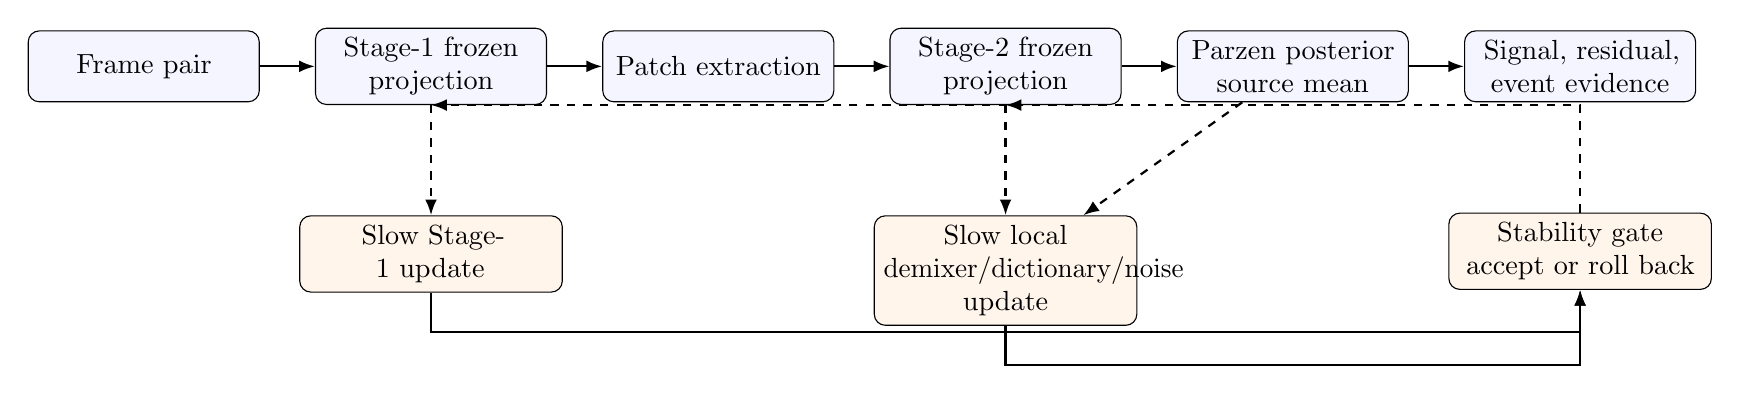
\begin{tikzpicture}[
  box/.style={draw,rounded corners,minimum height=9mm,text width=27mm,align=center,fill=blue!4},
  slow/.style={draw,rounded corners,minimum height=9mm,text width=31mm,align=center,fill=orange!8},
  arrow/.style={-{Latex[length=2mm]},thick},
  node distance=6mm and 7mm]
\node[box] (pair) {Frame pair};
\node[box,right=of pair] (bginf) {Stage-1 frozen\\projection};
\node[box,right=of bginf] (patch) {Patch extraction};
\node[box,right=of patch] (proj) {Stage-2 frozen\\projection};
\node[box,right=of proj] (post) {Parzen posterior\\source mean};
\node[box,right=of post] (out) {Signal, residual,\\event evidence};
\draw[arrow] (pair)--(bginf);
\draw[arrow] (bginf)--(patch);
\draw[arrow] (patch)--(proj);
\draw[arrow] (proj)--(post);
\draw[arrow] (post)--(out);

\node[slow,below=14mm of bginf] (s1up) {Slow Stage-1 update};
\node[slow,below=14mm of proj] (s2up) {Slow local demixer/dictionary/noise update};
\node[slow,below=14mm of out] (guard) {Stability gate\\accept or roll back};
\draw[arrow,dashed] (bginf)--(s1up);
\draw[arrow,dashed] (proj)--(s2up);
\draw[arrow,dashed] (post)--(s2up);
\draw[arrow] (s1up.south) -- ++(0,-5mm) -| (guard.south);
\draw[arrow] (s2up.south) -- ++(0,-5mm) -| (guard.south);
\draw[arrow,dashed] (guard.north) |- (bginf.south);
\draw[arrow,dashed] (guard.north) |- (proj.south);
\end{tikzpicture}%
}
\caption{Two-timescale implementation. The fast path performs fixed inference;
slow updates are checkpointed, tested, and either accepted or rolled back.}
\label{fig:realtime}
\end{figure}

\section{Falsification-oriented evaluation}

\subsection{Synthetic and semi-synthetic construction}

Generate exact channels $B,S,A,N$ using:
\begin{itemize}[leftmargin=*]
\item static, gain-varying, linearly drifting, and nonlinear backgrounds;
\item localized disks and membrane-like annuli;
\item fast transients, slow ramps, plateaus, and overlapping events;
\item independent and synchronous sources;
\item translations, edge motion, saturation, and impulsive artifacts;
\item white, correlated, heteroscedastic, and Poisson--Gaussian noise;
\item patch-boundary and image-boundary cases.
\end{itemize}
Semi-synthetic experiments inject exact sources and artifacts into real quiet
NeuRev frames while retaining every ground-truth channel.

\subsection{Decomposition metrics}

The closure error is
\begin{equation}
\mathcal E_{\mathrm{closure}}
=
\frac{\norm{Y-\widehat B-\widehat S-\widehat A-\widehat N}_F^2}
{\norm{Y}_F^2+\epsilon}.
\end{equation}
For true channel $C_i$ and estimated channel $\widehat C_j$, report a leakage
matrix
\begin{equation}
L_{ij}
=
\frac{\norm{\operatorname{Proj}_{\widehat C_j}(C_i)}_F^2}
{\norm{C_i}_F^2+\epsilon},
\end{equation}
plus direct NMSE and aligned correlation because projection metrics can favor
high-rank channels.

\subsection{Event preservation}

For each known or injected event, report:
\begin{itemize}[leftmargin=*]
\item amplitude ratio and temporal-area ratio;
\item onset, peak, and duration error;
\item centroid error and footprint/annulus overlap;
\item energy moved into background, artifact, and noise;
\item local signal-to-quiet evidence before and after each stage.
\end{itemize}

\subsection{Residual validity}

Report temporal ACF, spatial correlation versus distance, power spectrum,
intensity-conditioned variance, tail behavior, event-triggered residual average,
and correlation with gradients/motion. A residual that contains coherent
membrane structure is missed signal; a residual with moving paired edges is
artifact; a residual with smooth global fluctuations is missed background.

\subsection{Downstream NeuRev metrics}

Use identical temporal pooling, quiet calibration, NMS, matching, and candidate
budgets across lanes. Compare both recall-versus-candidate burden and fixed-budget
recall. Unmatched candidates remain unknown. Add annular/footprint-aware matching
and pre-NMS versus post-NMS audits so representation failure is separated from
detector failure.

\section{Mandatory result figures}

The implementation package requires the following outputs:

\begin{table}[H]
\centering
\small
\begin{tabularx}{\textwidth}{>{\raggedright\arraybackslash}p{0.22\textwidth}X}
\toprule
Figure & Required content \\
\midrule
Decomposition sheet & Raw, background, Stage-1 residual, neural signal, artifact,
noise, sum reconstruction, closure error at quiet/event/shared-miss/artifact frames. \\
Stage-1 geometry & Pair cloud, common/difference directions, fitted axes,
classification confidence, angle and identity tracking. \\
Staticness scatter & First- vs second-derivative energy, spatial broadness,
common-direction cosine, resolved/unresolved labels. \\
Noise spectrum & Residual covariance, estimated noise, positive
$\Sigma_r-\Sigma_n$ spectrum, selected rank and block stability. \\
Parzen diagnostics & Dictionary centers, clean and noise-convolved densities,
projected noise, score, posterior shrinkage curve. \\
Component galleries & Spatial maps, noisy/clean traces, morphology, motion
correlation, stability, acceptance reason. \\
Leakage matrix & True $B/S/A/N$ versus estimated $B/S/A/N$ with uncertainty. \\
Residual diagnostics & ACF, spatial correlation, PSD, intensity-variance,
event-triggered residual, gradient/motion correlation. \\
Event preservation & Amplitude/area/timing/morphology/leakage distributions and
paired shared-miss traces. \\
Detection Pareto & Known-label recall versus candidate burden and fixed-budget
recall for all anchors and proposed lanes. \\
Shared failures & Observation-by-method matrix separating representation,
threshold, NMS, matching, annotation, and no-evidence failures. \\
Stability & Demixer angles, component correlations, candidate Jaccard, leakage
variation over seeds/windows/patch offsets/ranks. \\
Latency & Stage and total p50/p95/p99, memory, adaptation frequency, fallback
count, and 20 ms deadline. \\
\bottomrule
\end{tabularx}
\caption{Mandatory visual evidence. Conceptual diagrams in this manuscript are
not substitutes for experiment-generated figures.}
\label{tab:figures}
\end{table}

\section{Stage gates}

\begin{enumerate}[leftmargin=*,label=\textbf{C\arabic*:}]
\item \textbf{Implementation integrity.} Deterministic tests, exact closure,
collision-safe artifacts, correct frames/coordinates, and Raw Direct anchor.
\item \textbf{Stage-1 identifiability and stability.} Finite conditioning,
continuous component identity, bounded updates, and unresolved fallback.
\item \textbf{Stage-1 scientific validity.} Low signal leakage into background,
background reduction beyond fixed subtraction, and slow-event preservation.
\item \textbf{Stage-2 numerical stability.} PSD covariance, stable rank, bounded
noise variance/dictionaries, stable demixing, overlap-add closure.
\item \textbf{Stage-2 decomposition validity.} Better source recovery than
noise-agnostic ICA and a less structured residual without artifact relabeling.
\item \textbf{Real signal preservation.} Stable amplitude, area, timing,
morphology, and localization on real known events and reviewed failures.
\item \textbf{Downstream value.} Improved held-out recall in at least three of
four bursts or at least 20\% candidate reduction without recall loss.
\item \textbf{Real-time candidacy.} Frozen causal inference below 20 ms at p95,
with safe slow-update freeze/rollback behavior.
\end{enumerate}
No later gate is valid when an upstream gate is incomplete.

\section{Principal risks}

\begin{table}[H]
\centering
\small
\begin{tabularx}{\textwidth}{>{\raggedright\arraybackslash}p{0.23\textwidth}
                             >{\raggedright\arraybackslash}X
                             >{\raggedright\arraybackslash}X}
\toprule
Risk & Failure mechanism & Required response \\
\midrule
Slow signal absorbed as background & Low derivative energy resembles persistent
background & Staticness margin, spatial/morphology terms, unresolved state,
semi-synthetic slow ramps, alternating refinement. \\
Stage-1 error propagation & Removed signal is unavailable to Stage 2 & Preserve
raw/background/residual, measure leakage, confidence-weighted/fallback lane,
optional one-pass refinement. \\
Noise treated as source & Gaussian noise is rotationally ambiguous & Explicit
noise covariance, noise-corrected subspace, posterior source estimator, residual
qualification. \\
Structured artifact accepted & Motion/saturation are non-Gaussian and coherent &
Artifact class, motion/gradient/saturation features, review gallery. \\
Parzen collapse or saturation & Bandwidth/dictionary/update degeneracy & Bounds,
leave-one-out, dictionary diagnostics, finite-difference tests, rollback. \\
High-rank instability & Too many components and weak identifiability & Local
patches, bounded rank, seed/window stability, stop gates. \\
False confidence from detection & More candidates can raise recall & Fixed-budget
comparison, sparse-positive semantics, shared-failure audit. \\
Real-time drift & Continual adaptation changes component meaning & Fast frozen
path, slow checkpointed updates, sign/permutation tracking, fallback. \\
\bottomrule
\end{tabularx}
\caption{Dominant failure modes and the corresponding implementation safeguards.}
\end{table}

\section{Conclusion}

The proposed hierarchy is viable as a bounded research program, not as an
assumption that two consecutive ICA calls automatically identify background,
neurons, and noise. Stage~1 should use Parzen ICA to estimate a common/background
mode and reconstruct an amplitude-preserving residual. Stage~2 should use local
multichannel patches, an explicit noise covariance, a source density convolved
with the projected noise distribution, a stochastic score-function update, and
posterior source denoising. Coherent components must then be classified as
neural, artifact, or unresolved before the final residual is called measurement
noise.

The information-theoretic contribution is precise: Parzen densities provide a
nonparametric score for adaptive separation; stochastic information-gradient
updates provide a bounded online route; and noise convolution converts the same
source model into a denoising posterior. The scientific contribution depends on
closure, leakage, event preservation, residual validity, stability, and real-time
behavior---not on entropy reduction alone.

\begin{thebibliography}{99}

\bibitem{bell1995infomax}
A.~J. Bell and T.~J. Sejnowski,
``An information-maximization approach to blind separation and blind
deconvolution,''
\emph{Neural Computation}, vol.~7, no.~6, pp.~1129--1159, 1995.

\bibitem{erdogmus2003sig}
D.~Erdogmus, K.~E. Hild II, and J.~C. Principe,
``Online entropy manipulation: Stochastic information gradient,''
\emph{IEEE Signal Processing Letters}, vol.~10, no.~8, pp.~242--245, 2003.

\bibitem{erdogmus2004deconvolution}
D.~Erdogmus, K.~E. Hild II, J.~C. Principe, M.~L\'azaro, and I.~Santamar\'ia,
``Adaptive blind deconvolution of linear channels using R\'enyi's entropy with
Parzen window estimation,''
\emph{IEEE Transactions on Signal Processing}, vol.~52, no.~6,
pp.~1489--1498, 2004.

\bibitem{hild2006entropy}
K.~E. Hild II, D.~Erdogmus, and J.~C. Principe,
``An analysis of entropy estimators for blind source separation,''
\emph{Signal Processing}, vol.~86, no.~1, pp.~182--194, 2006.

\bibitem{yang2007adaptive}
J.-M. Yang and H.~Sakai,
``A new adaptive filter algorithm for system identification using independent
component analysis,''
\emph{IEICE Transactions on Fundamentals of Electronics, Communications and
Computer Sciences}, vol.~E90-A, no.~8, pp.~1549--1554, 2007.

\bibitem{voss2015pegi}
J.~R. Voss, M.~Belkin, and L.~Rademacher,
``A pseudo-Euclidean iteration for optimal recovery in noisy ICA,''
in \emph{Advances in Neural Information Processing Systems 28},
pp.~2872--2880, 2015.

\bibitem{pnevmatikakis2016cnmf}
E.~A. Pnevmatikakis \emph{et al.},
``Simultaneous denoising, deconvolution, and demixing of calcium imaging data,''
\emph{Neuron}, vol.~89, no.~2, pp.~285--299, 2016.

\bibitem{friedrich2017oasis}
J.~Friedrich, P.~Zhou, and L.~Paninski,
``Fast online deconvolution of calcium imaging data,''
\emph{PLoS Computational Biology}, vol.~13, no.~3, e1005423, 2017.

\bibitem{buchanan2018pmd}
E.~K. Buchanan \emph{et al.},
``Penalized matrix decomposition for denoising, compression, and improved
demixing of functional imaging data,''
\emph{arXiv preprint arXiv:1807.06203}, 2018.

\end{thebibliography}

\end{document}
